\documentclass[man,floatsintext,draftall]{apa6}
\usepackage{lmodern}
\usepackage{amssymb,amsmath}
\usepackage{ifxetex,ifluatex}
\usepackage{fixltx2e} % provides \textsubscript
\ifnum 0\ifxetex 1\fi\ifluatex 1\fi=0 % if pdftex
  \usepackage[T1]{fontenc}
  \usepackage[utf8]{inputenc}
\else % if luatex or xelatex
  \ifxetex
    \usepackage{mathspec}
  \else
    \usepackage{fontspec}
  \fi
  \defaultfontfeatures{Ligatures=TeX,Scale=MatchLowercase}
\fi
% use upquote if available, for straight quotes in verbatim environments
\IfFileExists{upquote.sty}{\usepackage{upquote}}{}
% use microtype if available
\IfFileExists{microtype.sty}{%
\usepackage{microtype}
\UseMicrotypeSet[protrusion]{basicmath} % disable protrusion for tt fonts
}{}
\usepackage{hyperref}
\hypersetup{unicode=true,
            pdftitle={The production of negation in parents' and children's speech},
            pdfauthor={First Author~\& Ernst-August Doelle},
            pdfkeywords={keywords},
            pdfborder={0 0 0},
            breaklinks=true}
\urlstyle{same}  % don't use monospace font for urls
\usepackage{graphicx,grffile}
\makeatletter
\def\maxwidth{\ifdim\Gin@nat@width>\linewidth\linewidth\else\Gin@nat@width\fi}
\def\maxheight{\ifdim\Gin@nat@height>\textheight\textheight\else\Gin@nat@height\fi}
\makeatother
% Scale images if necessary, so that they will not overflow the page
% margins by default, and it is still possible to overwrite the defaults
% using explicit options in \includegraphics[width, height, ...]{}
\setkeys{Gin}{width=\maxwidth,height=\maxheight,keepaspectratio}
\IfFileExists{parskip.sty}{%
\usepackage{parskip}
}{% else
\setlength{\parindent}{0pt}
\setlength{\parskip}{6pt plus 2pt minus 1pt}
}
\setlength{\emergencystretch}{3em}  % prevent overfull lines
\providecommand{\tightlist}{%
  \setlength{\itemsep}{0pt}\setlength{\parskip}{0pt}}
\setcounter{secnumdepth}{0}
% Redefines (sub)paragraphs to behave more like sections
\ifx\paragraph\undefined\else
\let\oldparagraph\paragraph
\renewcommand{\paragraph}[1]{\oldparagraph{#1}\mbox{}}
\fi
\ifx\subparagraph\undefined\else
\let\oldsubparagraph\subparagraph
\renewcommand{\subparagraph}[1]{\oldsubparagraph{#1}\mbox{}}
\fi

%%% Use protect on footnotes to avoid problems with footnotes in titles
\let\rmarkdownfootnote\footnote%
\def\footnote{\protect\rmarkdownfootnote}


  \title{The production of negation in parents' and children's speech}
<<<<<<< HEAD
    \author{First Author\textsuperscript{1}~\& Ernst-August
Doelle\textsuperscript{1,2}}
=======
    \author{First Author\textsuperscript{1}~\& Ernst-August Doelle\textsuperscript{1,2}}
>>>>>>> 9cd6424fe63fc80f114c1ca04fb952c90eaf9aee
    \date{}
  
\shorttitle{Child and Parent Production of Negation}
\affiliation{
\vspace{0.5cm}
\textsuperscript{1} Wilhelm-Wundt-University\\\textsuperscript{2} Konstanz Business School}
\keywords{keywords\newline\indent Word count: X}
\usepackage{csquotes}
\usepackage{upgreek}
\captionsetup{font=singlespacing,justification=justified}

\usepackage{longtable}
\usepackage{lscape}
\usepackage{multirow}
\usepackage{tabularx}
\usepackage[flushleft]{threeparttable}
\usepackage{threeparttablex}

\newenvironment{lltable}{\begin{landscape}\begin{center}\begin{ThreePartTable}}{\end{ThreePartTable}\end{center}\end{landscape}}

\makeatletter
\newcommand\LastLTentrywidth{1em}
\newlength\longtablewidth
\setlength{\longtablewidth}{1in}
\newcommand{\getlongtablewidth}{\begingroup \ifcsname LT@\roman{LT@tables}\endcsname \global\longtablewidth=0pt \renewcommand{\LT@entry}[2]{\global\advance\longtablewidth by ##2\relax\gdef\LastLTentrywidth{##2}}\@nameuse{LT@\roman{LT@tables}} \fi \endgroup}


\usepackage{lineno}

\linenumbers

\authornote{Add complete departmental affiliations for each author here. Each new line herein must be indented, like this line.

Enter author note here.

Correspondence concerning this article should be addressed to First Author, Postal address. E-mail: \href{mailto:my@email.com}{\nolinkurl{my@email.com}}}

\abstract{
this is the abstract


}

\begin{document}
\maketitle

\hypertarget{introduction}{%
\section{Introduction}\label{introduction}}

Children start producing all types of English negation by age 18 months and by 36 months, they produce them at the rate parents do.
types of negation in English: no, verbal (not, nt), lexical (nothing, nobody, nowhere, none, un-in-de-dis-).

Study 1 Questions
* What is the overall trajectory of negative forms in child production?
* Does the development of negation follow a no \textgreater{} not \textgreater{} nt cline? (Cameron-faulkner et al)
* How many children are found to produce no/not/nt at each age?
* Do positive variants of the negative constructions exist too?
* Are early \enquote{can't} and \enquote{don't} examples unanalyzed wholes? (Klima \& Bellugi 1966; Bloom 1970) Do children produce \enquote{can't} and \enquote{don't} before using \enquote{do} and \enquote{can}?
* Proportion of no vs.~not vs.~nt broken down by mean length of utterance
* instead of age, put mean length of utterance on the x axis?

Study 2 Questions
* What are early constructions?
* the response may differ based on annotation level
* Do children's early negative utterances differ so much from those used by adults? (Thornton \& Tesan 2013)
* How common are ungrammatical non-adult like combinations?
* How many pre-sentential negation? (NEG + Subject + Predicate)
* How many sentence internal? (Subj + NEG + Predicate)
* Is negation external at the beginning? (appear before subjects) Does a NEG + S schema mark the beginning of negation? (McNeill \& McNeill)
* How many are optional infinitive: it not fit in here, it don't fit in here?
* control MLU: which forms are common among 1/2/3/\ldots{} word utterances?
* exclude single \enquote{no} (as well as anaphoric no) utterances from \enquote{no + more words}
* What is anaphoric negation negating?
* How productive are early forms of negation?
* average neg + \#WORD per child as measure of productivity

\hypertarget{previous-studies}{%
\subsection{Previous Studies}\label{previous-studies}}

<<<<<<< HEAD
Claim: Children start producing all types of English negation by age 18
months and by 36 months, they produce them at the rate parents do. types
of negation in English: no, verbal (not, nt), lexical (nothing, nobody,
nowhere, none, un-in-de-dis-).

Study 1 Questions * What is the overall trajectory of negative forms in
child production? * Does the development of negation follow a no
\textgreater{} not \textgreater{} nt cline? (Cameron-faulkner et al) *
How many children are found to produce no/not/nt at each age? * Do
positive variants of the negative constructions exist too? * Are early
\enquote{can't} and \enquote{don't} examples unanalyzed wholes? (Klima
\& Bellugi 1966; Bloom 1970) Do children produce \enquote{can't} and
\enquote{don't} before using \enquote{do} and \enquote{can}? *
Proportion of no vs.~not vs.~nt broken down by mean length of utterance
* instead of age, put mean length of utterance on the x axis?

Study 2 Questions * What are early constructions? * the response may
differ based on annotation level * Do children's early negative
utterances differ so much from those used by adults? (Thornton \& Tesan
2013) * How common are ungrammatical non-adult like combinations? * How
many pre-sentential negation? (NEG + Subject + Predicate) * How many
sentence internal? (Subj + NEG + Predicate) * Is negation external at
the beginning? (appear before subjects) Does a NEG + S schema mark the
beginning of negation? (McNeill \& McNeill) * How many are optional
infinitive: it not fit in here, it don't fit in here? * control MLU:
which forms are common among 1/2/3/\ldots{} word utterances? * exclude
single \enquote{no} (as well as anaphoric no) utterances from
\enquote{no + more words} * What is anaphoric negation negating? * How
productive are early forms of negation? * average neg + \#WORD per child
as measure of productivity

\subsection{Previous Studies}\label{previous-studies}
=======
Formal and functional development of negation

\begin{enumerate}
\def\labelenumi{\arabic{enumi}.}
\item
  Klima \& Bellugi. 1966. Syntactic regularities in the speech of children. In Psycholinguistic papers, ed. J. Lyons and R. Wales, 183-208. Edinburgh: Edinburgh University Press.
\item
  Bellugi (1967). The acquisition of negation. Doctoral dissertation, Harvard University, Cambridge, Mass.
\item
  McNeill \& McNeill 1968: Japanese
\item
  Bloom, L. (1970). Language development: Form and function in emerging grammars. Cambridge, MA: MIT Press.
\item
  Lord (1974): Variations in the pattern of acquisition of negation
\item
  Wode, H. (1977). Four early stages in the development of L1 negation. Journal of Child Language 4, 87--102.
\item
  Pea (1978): the development of negation in early child language. dissertation
\item
  De Villiers, P., and J. G. De Villiers (1979) \enquote{Form and function in the development of sentence negation}, Papers and Reports on Child Language Development, 17, 57- 64.
\item
  Pea Dissertation
\item
  Clahsen, Harald. 1983. Some remarks on the acquisition of German negation. Journal of Child Language 10:465-469.
\item
  Choi, S. (1988). The semantic development of negation: A cross-linguistic longitudinal study. Journal of Child Language, 15, 517--531.
\item
  Weissenborn, Juirgen, and Monica Verrips. 1989. Negation as a window to the structure of early child language. Ms., Max Planck Institut fur Psycholinguistik, Nijmegen.
\item
  Deprez, Viviane and Amy Pierce. 1993. Negation and Functional Projections in Early Grammar. Linguistic Inquiry 24, no. 1: 25-67.
\item
  Stromswold, K. (1997) The Acquisition of Inversion and Negation in English: A Reply to Deprez and Pierce', ms. Rutgers.
\item
  Drozd (1995): Child English pre-sentential negation as metalinguistic exclamatory sentence negation. JCL
\item
  Hamann 2000
\item
  Cameron-Faulkner, T., Lieven, E., \& Theakston, A. (2007). What part of no do children not understand? A usage-based account of multiword negation. Journal of Child Language, 34, 251--282.
\item
  Guidetti (2000): Pragmatic study of agreement and refusal messages in young French children. Journal of Pragmatics
\item
  Guidetti (2005): Yes or no? How young French children combinegestures and speech to agree and refuse. JCL
\item
  Schutze (2010) The Status of Nonagreeing Don't and Theories of Root Infinitives
\item
  Dimroth (2010): The Acquisition of Negation
\item
  Thornton \& Tesan (2013): sentential negation in early child English
\item
  Nordmeyer \& Frank (2014): Individual variation in children's early production of negation
\end{enumerate}

\hypertarget{current-study}{%
\subsection{Current Study}\label{current-study}}
>>>>>>> 9cd6424fe63fc80f114c1ca04fb952c90eaf9aee

Acquisition of negation should concern itself with two notions: 1. negative morpheme 2. compositional complexity. By negative morpheme, we mean the kinds of morphemes that at each stage of acquisition are mapped to negative meanings. English has adverbal and adnominal mophemes that encode the concept of negation. We can look at how each form-meaning mapping emerges in children's development. Second by compositional complexity, we mean the types of elements that each morphemes succesfully negates at each stage of development. Under stuch analysis negation may have been successfully acquired to operate on locative elements but not identity relations. Compositional complexity of negation at each stage also helps us understand how quickly children generalize the function of negation beyond specific arguments it takes in the child's input.

<<<<<<< HEAD
\subsection{Current Study}\label{current-study}

Acquisition of negation should concern itself with two notions: 1.
negative morpheme 2. compositional complexity. By negative morpheme, we
mean the kinds of morphemes that at each stage of acquisition are mapped
to negative meanings. English has adverbal and adnominal mophemes that
encode the concept of negation. We can look at how each form-meaning
mapping emerges in children's development. Second by compositional
complexity, we mean the types of elements that each morphemes
succesfully negates at each stage of development. Under stuch analysis
negation may have been successfully acquired to operate on locative
elements but not identity relations. Compositional complexity of
negation at each stage also helps us understand how quickly children
generalize the function of negation beyond specific arguments it takes
in the child's input.

\section{Study 1: Large-scale
metrics}\label{study-1-large-scale-metrics}

\subsection{Methods}\label{methods}

For samples of parents' and children's speech, we used the online
database \href{childes-db.stanford.edu}{childes-db} and its associated R
programming package \texttt{childesr} ({\textbf{???}}). Childes-db is an
online interface to the child language components of
\href{https://talkbank.org/}{TalkBank}, namely
\href{https://childes.talkbank.org/}{CHILDES} ({\textbf{???}}) and
\href{https://phonbank.talkbank.org/}{PhonBank}. Two collections of
corpora were selected: English-North America and English-UK.

\subsubsection{Procedure}\label{procedure}

All word tokens were tagged for the following information: 1. The
speaker role (parent vs.~child), 2. the age of the child when the word
was produced, 3. the type of the utterance the word appeared in
(declarative, question, imperative, other)\footnote{This study grouped
  utterance types into four main categories: \enquote{declarative},
  \enquote{question}, \enquote{imperative}, and \enquote{other}.
  Utterance type categorization followed the convention used in the
  \href{https://talkbank.org/manuals/CHAT.html\#_Toc486414422}{TalkBank
  manual}. The utterance types are similar to sentence types
  (declarative, interrogative, imperative) with one exception: the
  category \enquote{question} consists of interrogatives as well as
  rising declaratives (i.e.~declaratives with rising question
  intonation). In the transcripts, declaratives are marked with a
  period, questions with a question mark, and imperatives with an
  exclamation mark. It is important to note that the manual also
  provides
  \href{https://talkbank.org/manuals/CHAT.html\#_Toc486414431}{terminators
  for special-type utterances}. Among the special type utterances, this
  study included the following in the category \enquote{questions}:
  trailing off of a question, question with exclamation, interruption of
  a question, and self-interrupted question. The category imperatives
  also included \enquote{emphatic imperatives}. The rest of the special
  type utterances such as \enquote{interruptions} and \enquote{trailing
  off} were included in the category \enquote{other}.}, 4. whether the
word was positive or negative, and 5. the type of negative word
produced. For this study we considerd the following classes of negative
words in English: the words \emph{no} and \emph{not}, the negative
clitic auxiliary forms with \emph{nt} (\emph{ain't}, \emph{isn't},
\emph{amn't}, \emph{aren't}, \emph{wasn't}, \emph{weren't},
\emph{don't}, \emph{doesn't}, \emph{didn't}, \emph{won't},
\emph{shan't}, \emph{hasn't}, \emph{havn't}, \emph{hadn't},
\emph{shouldn't}, \emph{can't}, \emph{couldn't}, \emph{may'nt},
\emph{might'nt}, \emph{would'nt}, and \emph{mustn't}), negative
quantifiers or adverbs of frequency (\emph{nothing}, \emph{nobody},
\emph{nowhere}, \emph{no-one}, \emph{none}, \emph{never}), as well as
derivational negative forms with morphemes \emph{un-} (e.g.~unhappy),
\emph{in-} (e.g.~invisible), \emph{dis-}(e.g.~disappear), \emph{de-}
(e.g.~defrost), \emph{non-} (e.g.~nonsense), and \emph{-less}
(e.g.~careless).

\subsubsection{Exclusion Criteria}\label{exclusion-criteria}

\subsection{Results}\label{results}

\subsection{Conclusions}\label{conclusions}

\section{Study 2: Early Productions}\label{study-2-early-productions}

Participant information: 1. what is the distribution of words per
participant? 2. what proportion of children in each monthly age bin
produce negative morphemes?

Filtering Process: (In parentheses I haven't done yet) 1. New column
(condensed\_p\_o\_s) transformations: nouns, proper nouns, pronouns
-\textgreater{} n (no -\textgreater{} no (replacing co/qn); haven't done
this yet) all types of adverbs and determiners condensed to adv and det
respectively (no n n -\textgreater{} no v n: no cockle me no hug baby no
it's yours no brush hair no ride horsie no stop it no help me no spin it
no touch Lastname no pop weasel no play toys no pinch that no hold it)
(no n n -\textgreater{} no n v: no Mommy Humm no mummy sneeze no phone
talk no everybody fall no hair wash) (no n n -\textgreater{} no adj n:
no tomato soup no clam chowder no Pat's hat no ice pop) 2. filtered to
constructions that occur at least 10 times 3. filtered out \enquote{no},
\enquote{no no}, \enquote{no no no}, \enquote{no no no no}, and
\enquote{}

\subsection{Participants}\label{participants}

\subsection{Material}\label{material}

\subsection{Procedure}\label{procedure-1}

\subsection{Data analysis}\label{data-analysis}

\begin{longtable}[]{@{}ll@{}}
\toprule
Abbreviation & Meaning\tabularnewline
\midrule
\endhead
n & noun (includes pronouns and proper nouns)\tabularnewline
v & verb\tabularnewline
adj & adjective\tabularnewline
adv & adverb\tabularnewline
prep & preposition\tabularnewline
det & determiner\tabularnewline
part & participle\tabularnewline
mod & modal\tabularnewline
\bottomrule
\end{longtable}

\begin{longtable}[]{@{}lll@{}}
\toprule
\begin{minipage}[b]{0.23\columnwidth}\raggedright\strut
Construction\strut
\end{minipage} & \begin{minipage}[b]{0.15\columnwidth}\raggedright\strut
Frequency\strut
\end{minipage} & \begin{minipage}[b]{0.47\columnwidth}\raggedright\strut
Examples\strut
\end{minipage}\tabularnewline
\midrule
\endhead
\begin{minipage}[t]{0.23\columnwidth}\raggedright\strut
no n\strut
\end{minipage} & \begin{minipage}[t]{0.15\columnwidth}\raggedright\strut
455\strut
\end{minipage} & \begin{minipage}[t]{0.47\columnwidth}\raggedright\strut
no baby, no horsie, no juice\strut
\end{minipage}\tabularnewline
\begin{minipage}[t]{0.23\columnwidth}\raggedright\strut
mod v n\strut
\end{minipage} & \begin{minipage}[t]{0.15\columnwidth}\raggedright\strut
142\strut
\end{minipage} & \begin{minipage}[t]{0.47\columnwidth}\raggedright\strut
don't touch that, don't fit car, can't open it\strut
\end{minipage}\tabularnewline
\begin{minipage}[t]{0.23\columnwidth}\raggedright\strut
n mod v n\strut
\end{minipage} & \begin{minipage}[t]{0.15\columnwidth}\raggedright\strut
90\strut
\end{minipage} & \begin{minipage}[t]{0.47\columnwidth}\raggedright\strut
I don't want juice, I can't find duck, cow won't go Mama\strut
\end{minipage}\tabularnewline
\begin{minipage}[t]{0.23\columnwidth}\raggedright\strut
no qn n\strut
\end{minipage} & \begin{minipage}[t]{0.15\columnwidth}\raggedright\strut
83\strut
\end{minipage} & \begin{minipage}[t]{0.47\columnwidth}\raggedright\strut
no more stuff, *no car, no no pram, no like doggy\strut
\end{minipage}\tabularnewline
\begin{minipage}[t]{0.23\columnwidth}\raggedright\strut
mod\strut
\end{minipage} & \begin{minipage}[t]{0.15\columnwidth}\raggedright\strut
74\strut
\end{minipage} & \begin{minipage}[t]{0.47\columnwidth}\raggedright\strut
don't, can't\strut
\end{minipage}\tabularnewline
\begin{minipage}[t]{0.23\columnwidth}\raggedright\strut
n mod v\strut
\end{minipage} & \begin{minipage}[t]{0.15\columnwidth}\raggedright\strut
73\strut
\end{minipage} & \begin{minipage}[t]{0.47\columnwidth}\raggedright\strut
I don't know, they don't fit, I can't open\strut
\end{minipage}\tabularnewline
\begin{minipage}[t]{0.23\columnwidth}\raggedright\strut
mod v\strut
\end{minipage} & \begin{minipage}[t]{0.15\columnwidth}\raggedright\strut
67\strut
\end{minipage} & \begin{minipage}[t]{0.47\columnwidth}\raggedright\strut
don't go, doesn't work, can't catch\strut
\end{minipage}\tabularnewline
\begin{minipage}[t]{0.23\columnwidth}\raggedright\strut
no n n\strut
\end{minipage} & \begin{minipage}[t]{0.15\columnwidth}\raggedright\strut
63\strut
\end{minipage} & \begin{minipage}[t]{0.47\columnwidth}\raggedright\strut
no baby bubble, no this one, *no brush hair\strut
\end{minipage}\tabularnewline
\begin{minipage}[t]{0.23\columnwidth}\raggedright\strut
n mod\strut
\end{minipage} & \begin{minipage}[t]{0.15\columnwidth}\raggedright\strut
55\strut
\end{minipage} & \begin{minipage}[t]{0.47\columnwidth}\raggedright\strut
I can't, Jane doesn't, mine didn't\strut
\end{minipage}\tabularnewline
\begin{minipage}[t]{0.23\columnwidth}\raggedright\strut
not n\strut
\end{minipage} & \begin{minipage}[t]{0.15\columnwidth}\raggedright\strut
39\strut
\end{minipage} & \begin{minipage}[t]{0.47\columnwidth}\raggedright\strut
not noodle, not home, not right\strut
\end{minipage}\tabularnewline
\begin{minipage}[t]{0.23\columnwidth}\raggedright\strut
no v\strut
\end{minipage} & \begin{minipage}[t]{0.15\columnwidth}\raggedright\strut
38\strut
\end{minipage} & \begin{minipage}[t]{0.47\columnwidth}\raggedright\strut
no read, no pooped, *no zipper\strut
\end{minipage}\tabularnewline
\begin{minipage}[t]{0.23\columnwidth}\raggedright\strut
no v n\strut
\end{minipage} & \begin{minipage}[t]{0.15\columnwidth}\raggedright\strut
33\strut
\end{minipage} & \begin{minipage}[t]{0.47\columnwidth}\raggedright\strut
no sit chair, no have cracker, no eat milk\strut
\end{minipage}\tabularnewline
\begin{minipage}[t]{0.23\columnwidth}\raggedright\strut
not adv\strut
\end{minipage} & \begin{minipage}[t]{0.15\columnwidth}\raggedright\strut
30\strut
\end{minipage} & \begin{minipage}[t]{0.47\columnwidth}\raggedright\strut
not today, not there, *not asleep\strut
\end{minipage}\tabularnewline
\begin{minipage}[t]{0.23\columnwidth}\raggedright\strut
n no\strut
\end{minipage} & \begin{minipage}[t]{0.15\columnwidth}\raggedright\strut
25\strut
\end{minipage} & \begin{minipage}[t]{0.47\columnwidth}\raggedright\strut
mammy no, apple no, train no\strut
\end{minipage}\tabularnewline
\begin{minipage}[t]{0.23\columnwidth}\raggedright\strut
no adv\strut
\end{minipage} & \begin{minipage}[t]{0.15\columnwidth}\raggedright\strut
24\strut
\end{minipage} & \begin{minipage}[t]{0.47\columnwidth}\raggedright\strut
no there, no up, no behind\strut
\end{minipage}\tabularnewline
\begin{minipage}[t]{0.23\columnwidth}\raggedright\strut
no n n n\strut
\end{minipage} & \begin{minipage}[t]{0.15\columnwidth}\raggedright\strut
24\strut
\end{minipage} & \begin{minipage}[t]{0.47\columnwidth}\raggedright\strut
no night night moon, no mummy this side, *no hold daddy hand\strut
\end{minipage}\tabularnewline
\begin{minipage}[t]{0.23\columnwidth}\raggedright\strut
mod v n n\strut
\end{minipage} & \begin{minipage}[t]{0.15\columnwidth}\raggedright\strut
22\strut
\end{minipage} & \begin{minipage}[t]{0.47\columnwidth}\raggedright\strut
don't eat skin part, (?) don't touch that book, *can't find bunny
rabit\strut
\end{minipage}\tabularnewline
\begin{minipage}[t]{0.23\columnwidth}\raggedright\strut
no prep n\strut
\end{minipage} & \begin{minipage}[t]{0.15\columnwidth}\raggedright\strut
19\strut
\end{minipage} & \begin{minipage}[t]{0.47\columnwidth}\raggedright\strut
no in tree, no with this, *no like bubbles\strut
\end{minipage}\tabularnewline
\begin{minipage}[t]{0.23\columnwidth}\raggedright\strut
n mod v prep\strut
\end{minipage} & \begin{minipage}[t]{0.15\columnwidth}\raggedright\strut
17\strut
\end{minipage} & \begin{minipage}[t]{0.47\columnwidth}\raggedright\strut
I don't want to, Laura don't want to\strut
\end{minipage}\tabularnewline
\begin{minipage}[t]{0.23\columnwidth}\raggedright\strut
mod n\strut
\end{minipage} & \begin{minipage}[t]{0.15\columnwidth}\raggedright\strut
15\strut
\end{minipage} & \begin{minipage}[t]{0.47\columnwidth}\raggedright\strut
can't tea, don't Mommy, didn't I\strut
\end{minipage}\tabularnewline
\begin{minipage}[t]{0.23\columnwidth}\raggedright\strut
n v no\strut
\end{minipage} & \begin{minipage}[t]{0.15\columnwidth}\raggedright\strut
15\strut
\end{minipage} & \begin{minipage}[t]{0.47\columnwidth}\raggedright\strut
doll sit no, I take no, Joana say no\strut
\end{minipage}\tabularnewline
\begin{minipage}[t]{0.23\columnwidth}\raggedright\strut
no n v n\strut
\end{minipage} & \begin{minipage}[t]{0.15\columnwidth}\raggedright\strut
15\strut
\end{minipage} & \begin{minipage}[t]{0.47\columnwidth}\raggedright\strut
no car go car, no comb want brush, no mummy do it\strut
\end{minipage}\tabularnewline
\begin{minipage}[t]{0.23\columnwidth}\raggedright\strut
not adj\strut
\end{minipage} & \begin{minipage}[t]{0.15\columnwidth}\raggedright\strut
15\strut
\end{minipage} & \begin{minipage}[t]{0.47\columnwidth}\raggedright\strut
not good, not dirty, not real\strut
\end{minipage}\tabularnewline
\begin{minipage}[t]{0.23\columnwidth}\raggedright\strut
not det n\strut
\end{minipage} & \begin{minipage}[t]{0.15\columnwidth}\raggedright\strut
15\strut
\end{minipage} & \begin{minipage}[t]{0.47\columnwidth}\raggedright\strut
not my car, not a cat, not a white\strut
\end{minipage}\tabularnewline
\begin{minipage}[t]{0.23\columnwidth}\raggedright\strut
not v n\strut
\end{minipage} & \begin{minipage}[t]{0.15\columnwidth}\raggedright\strut
15\strut
\end{minipage} & \begin{minipage}[t]{0.47\columnwidth}\raggedright\strut
not eat rocks, not have coffee, not green one\strut
\end{minipage}\tabularnewline
\begin{minipage}[t]{0.23\columnwidth}\raggedright\strut
no det n\strut
\end{minipage} & \begin{minipage}[t]{0.15\columnwidth}\raggedright\strut
13\strut
\end{minipage} & \begin{minipage}[t]{0.47\columnwidth}\raggedright\strut
no my turn, no a cow, no the hammer\strut
\end{minipage}\tabularnewline
\begin{minipage}[t]{0.23\columnwidth}\raggedright\strut
not v\strut
\end{minipage} & \begin{minipage}[t]{0.15\columnwidth}\raggedright\strut
13\strut
\end{minipage} & \begin{minipage}[t]{0.47\columnwidth}\raggedright\strut
not shush, not work, not blanket\strut
\end{minipage}\tabularnewline
\begin{minipage}[t]{0.23\columnwidth}\raggedright\strut
mod v adv\strut
\end{minipage} & \begin{minipage}[t]{0.15\columnwidth}\raggedright\strut
12\strut
\end{minipage} & \begin{minipage}[t]{0.47\columnwidth}\raggedright\strut
can't come in, don't fall down, doesn't fit here\strut
\end{minipage}\tabularnewline
\begin{minipage}[t]{0.23\columnwidth}\raggedright\strut
no n adv\strut
\end{minipage} & \begin{minipage}[t]{0.15\columnwidth}\raggedright\strut
12\strut
\end{minipage} & \begin{minipage}[t]{0.47\columnwidth}\raggedright\strut
no jacket on, no monkey there, *no lie down\strut
\end{minipage}\tabularnewline
\begin{minipage}[t]{0.23\columnwidth}\raggedright\strut
no n v\strut
\end{minipage} & \begin{minipage}[t]{0.15\columnwidth}\raggedright\strut
12\strut
\end{minipage} & \begin{minipage}[t]{0.47\columnwidth}\raggedright\strut
no mail came, no mummy go, no I wanted\strut
\end{minipage}\tabularnewline
\begin{minipage}[t]{0.23\columnwidth}\raggedright\strut
no part\strut
\end{minipage} & \begin{minipage}[t]{0.15\columnwidth}\raggedright\strut
12\strut
\end{minipage} & \begin{minipage}[t]{0.47\columnwidth}\raggedright\strut
no bouncing, no eating, no hurting\strut
\end{minipage}\tabularnewline
\begin{minipage}[t]{0.23\columnwidth}\raggedright\strut
v no n n\strut
\end{minipage} & \begin{minipage}[t]{0.15\columnwidth}\raggedright\strut
12\strut
\end{minipage} & \begin{minipage}[t]{0.47\columnwidth}\raggedright\strut
man no taste it (???)\strut
\end{minipage}\tabularnewline
\begin{minipage}[t]{0.23\columnwidth}\raggedright\strut
n not n\strut
\end{minipage} & \begin{minipage}[t]{0.15\columnwidth}\raggedright\strut
11\strut
\end{minipage} & \begin{minipage}[t]{0.47\columnwidth}\raggedright\strut
pizza not pizza, pizza not apples, that not knees\strut
\end{minipage}\tabularnewline
\begin{minipage}[t]{0.23\columnwidth}\raggedright\strut
no adj\strut
\end{minipage} & \begin{minipage}[t]{0.15\columnwidth}\raggedright\strut
11\strut
\end{minipage} & \begin{minipage}[t]{0.47\columnwidth}\raggedright\strut
no happy, no pretend, no brown\strut
\end{minipage}\tabularnewline
\bottomrule
\end{longtable}

\begin{longtable}[]{@{}lll@{}}
\toprule
\begin{minipage}[b]{0.27\columnwidth}\raggedright\strut
Semantic Category\strut
\end{minipage} & \begin{minipage}[b]{0.16\columnwidth}\raggedright\strut
Frequency\strut
\end{minipage} & \begin{minipage}[b]{0.39\columnwidth}\raggedright\strut
Examples\strut
\end{minipage}\tabularnewline
\midrule
\endhead
\begin{minipage}[t]{0.27\columnwidth}\raggedright\strut
Do\strut
\end{minipage} & \begin{minipage}[t]{0.16\columnwidth}\raggedright\strut
666\strut
\end{minipage} & \begin{minipage}[t]{0.39\columnwidth}\raggedright\strut
don't like it, I don't feel good, no do it Mummy\strut
\end{minipage}\tabularnewline
\begin{minipage}[t]{0.27\columnwidth}\raggedright\strut
Ability (can)\strut
\end{minipage} & \begin{minipage}[t]{0.16\columnwidth}\raggedright\strut
212\strut
\end{minipage} & \begin{minipage}[t]{0.39\columnwidth}\raggedright\strut
I can't find a blankie, can't eat, no no I can not do\strut
\end{minipage}\tabularnewline
\begin{minipage}[t]{0.27\columnwidth}\raggedright\strut
Desire (want)\strut
\end{minipage} & \begin{minipage}[t]{0.16\columnwidth}\raggedright\strut
148\strut
\end{minipage} & \begin{minipage}[t]{0.39\columnwidth}\raggedright\strut
Don't want to, no comb want brush, no want the baby\strut
\end{minipage}\tabularnewline
\begin{minipage}[t]{0.27\columnwidth}\raggedright\strut
Don't want\strut
\end{minipage} & \begin{minipage}[t]{0.16\columnwidth}\raggedright\strut
106\strut
\end{minipage} & \begin{minipage}[t]{0.39\columnwidth}\raggedright\strut
I don't want juice, don't want it, Laura don't want to\strut
\end{minipage}\tabularnewline
\begin{minipage}[t]{0.27\columnwidth}\raggedright\strut
No {[}simple thing{]}\strut
\end{minipage} & \begin{minipage}[t]{0.16\columnwidth}\raggedright\strut
528\strut
\end{minipage} & \begin{minipage}[t]{0.39\columnwidth}\raggedright\strut
no go, no stupid, no now, no baby\strut
\end{minipage}\tabularnewline
\begin{minipage}[t]{0.27\columnwidth}\raggedright\strut
Not {[}simple thing{]}\strut
\end{minipage} & \begin{minipage}[t]{0.16\columnwidth}\raggedright\strut
97\strut
\end{minipage} & \begin{minipage}[t]{0.39\columnwidth}\raggedright\strut
not bad, not write, not quite\strut
\end{minipage}\tabularnewline
\begin{minipage}[t]{0.27\columnwidth}\raggedright\strut
Not noun\strut
\end{minipage} & \begin{minipage}[t]{0.16\columnwidth}\raggedright\strut
39\strut
\end{minipage} & \begin{minipage}[t]{0.39\columnwidth}\raggedright\strut
not noodle, not Danny, not right\strut
\end{minipage}\tabularnewline
\begin{minipage}[t]{0.27\columnwidth}\raggedright\strut
Presentential (Optimistic)\strut
\end{minipage} & \begin{minipage}[t]{0.16\columnwidth}\raggedright\strut
76\strut
\end{minipage} & \begin{minipage}[t]{0.39\columnwidth}\raggedright\strut
no daddy eat, no eat lunch, no in tree, no Toto here\strut
\end{minipage}\tabularnewline
\begin{minipage}[t]{0.27\columnwidth}\raggedright\strut
Presentential (Pessimistic)\strut
\end{minipage} & \begin{minipage}[t]{0.16\columnwidth}\raggedright\strut
12\strut
\end{minipage} & \begin{minipage}[t]{0.39\columnwidth}\raggedright\strut
no Mommy read, no I wanted, no I sweep, no water go\strut
\end{minipage}\tabularnewline
\bottomrule
\end{longtable}

\section{Results}\label{results-1}
=======
\hypertarget{study-1-large-scale-metrics}{%
\section{Study 1: Large-scale metrics}\label{study-1-large-scale-metrics}}

\hypertarget{methods}{%
\subsection{Methods}\label{methods}}

For samples of parents' and children's speech, we used the online database \href{childes-db.stanford.edu}{childes-db} and its associated R programming package \texttt{childesr} (Sanchez et al., 2018). Childes-db is an online interface to the child language components of \href{https://talkbank.org/}{TalkBank}, namely \href{https://childes.talkbank.org/}{CHILDES} (MacWhinney, 2000) and \href{https://phonbank.talkbank.org/}{PhonBank}. Two collections of corpora were selected: English-North America and English-UK.

\hypertarget{procedure}{%
\subsubsection{Procedure}\label{procedure}}

All word tokens were tagged for the following information: 1. The speaker role (parent vs.~child), 2. the age of the child when the word was produced, 3. the type of the utterance the word appeared in (declarative, question, imperative, other)\footnote{This study grouped utterance types into four main categories: \enquote{declarative}, \enquote{question}, \enquote{imperative}, and \enquote{other}. Utterance type categorization followed the convention used in the \href{https://talkbank.org/manuals/CHAT.html\#_Toc486414422}{TalkBank manual}. The utterance types are similar to sentence types (declarative, interrogative, imperative) with one exception: the category \enquote{question} consists of interrogatives as well as rising declaratives (i.e.~declaratives with rising question intonation). In the transcripts, declaratives are marked with a period, questions with a question mark, and imperatives with an exclamation mark. It is important to note that the manual also provides \href{https://talkbank.org/manuals/CHAT.html\#_Toc486414431}{terminators for special-type utterances}. Among the special type utterances, this study included the following in the category \enquote{questions}: trailing off of a question, question with exclamation, interruption of a question, and self-interrupted question. The category imperatives also included \enquote{emphatic imperatives}. The rest of the special type utterances such as \enquote{interruptions} and \enquote{trailing off} were included in the category \enquote{other}.}, 4. whether the word was positive or negative, and 5. the type of negative word produced. For this study we considerd the following classes of negative words in English: the words \emph{no} and \emph{not}, all possible negative clitic auxiliary forms with \emph{n't} (i.e. \emph{ain't}, \emph{isn't}, \emph{amn't}, \emph{aren't}, \emph{wasn't}, \emph{weren't}, \emph{don't}, \emph{doesn't}, \emph{didn't}, \emph{won't}, \emph{shan't}, \emph{hasn't}, \emph{havn't}, \emph{hadn't}, \emph{shouldn't}, \emph{can't}, \emph{couldn't}, \emph{may'nt}, \emph{might'nt}, \emph{would'nt}, and \emph{mustn't}) as well as their positive forms without \emph{n't} as controls, negative quantifiers (\emph{nothing}, \emph{nobody}, \emph{no-one}, \emph{nowhere}, \emph{none}) and their positive existential and universal variants (\emph{something}, \emph{everything}, \emph{somebody}, \emph{everybody}, \emph{someone}, \emph{everyone}, \emph{somewhere}, \emph{everywhere}, \emph{some}, \emph{all}), adverb of frequency \emph{never} and its existential and universal variants (\emph{sometimes}, \emph{always}), and finally derivational negative forms with morphemes \emph{un-} (e.g.~unhappy), \emph{in-} (e.g.~invisible), \emph{dis-}(e.g.~disappear), \emph{de-} (e.g.~defrost), \emph{non-} (e.g.~nonsense), and \emph{-less} (e.g.~careless).

\hypertarget{exclusion-criteria}{%
\subsubsection{Exclusion Criteria}\label{exclusion-criteria}}

First, unintelligible tokens were excluded (N = 379,549). Second, tokens that had missing information on children's age were excluded (N = 1,060,766). Third, tokens outside the age range of 1 to 6 years were excluded (N = 658,207). The collection contained the speech of 570 children and their parents after the exclusions.

\hypertarget{results}{%
\subsection{Results}\label{results}}

Following Cameron-Faulkner, Lieven, and Theakston (2007), we first look at the proportions of different categories of negation in parents' and children's speech between the ages of 1-6 years. As the right panel on Figure \ref{fig:negationProportionPlot} shows, parents generally produce more instances of auxiliary contracted negation \emph{n't} than \emph{no}, and produce more instances of \emph{no} than \emph{not}. However between the ages of 12-18 months, almost all children's negative forms are instances of \emph{no}, with a few contracted auxiliary negatives like \emph{don't} and \emph{can't}. Between 18 to 36 months, children's instances of \emph{not} and its contracted form \emph{n't} increase rapidly until they reach the parents' level of production. Although, the rate of \emph{no} production always stays above the parents' level, probably because paretns' ask more questions from children than children from adults. Similar to Cameron-Faulkner et al. (2007) we find that children start productions of \emph{no} earlier than other forms. However, unlike their conclusions, we find that children start producing the verb phrase negation \emph{not} and its contracted form \emph{nt} around the same time.

\begin{figure}
\centering
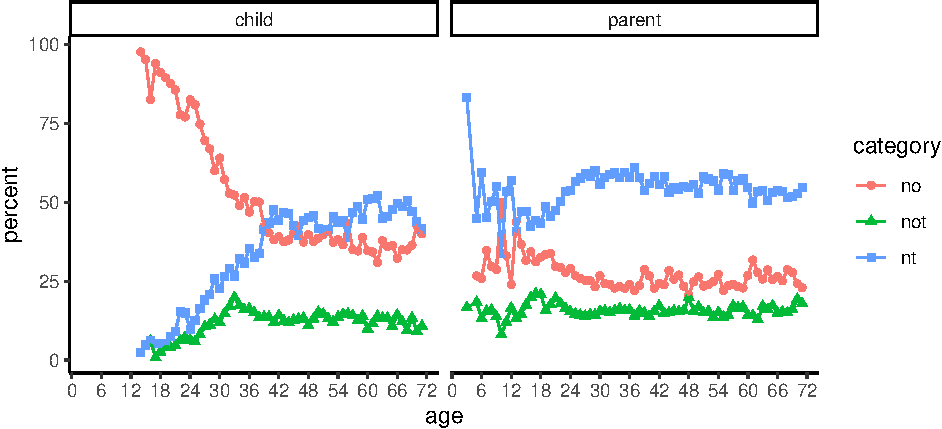
\includegraphics{negation_production_files/figure-latex/negationProportionPlot-1.pdf}
\caption{\label{fig:negationProportionPlot}Proportion of different categories of negation in parents' and children's speech between 1 to 6 years of age.}
\end{figure}

How does this interact with mean length of utterance? Are early \emph{no}'s mainly single word utterances?

\begin{figure}
\centering
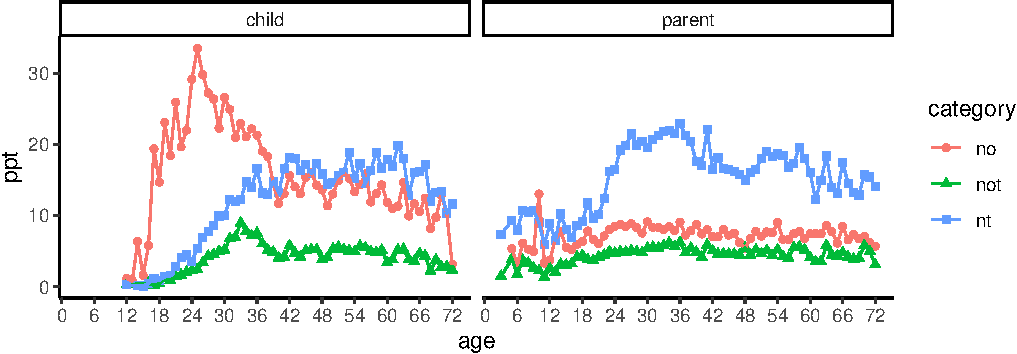
\includegraphics{negation_production_files/figure-latex/negationRelativeFrequency-1.pdf}
\caption{\label{fig:negationRelativeFrequency}Relative frequency of the response particle \emph{no}, verb phrase negation \emph{not}, and its contracted auxiliary forms like \emph{don't}}
\end{figure}

It is also often claimed in the literature (citation needed) that early forms of auxiliary negation like \emph{can't} and \emph{don't} are learned as unanalyzed chunks because the positive auxilliaries \emph{can} and \emph{do} are not produced at the same age. Figure (\ref{fig:auxRelFreq}) shows the relative frequency of positive and negative auxiliary forms in the speech of children and their parents. Our results show that overall, children start producing the positive and negative auxiliary forms around the same time and they always produce the positive forms at a higher rate than negative ones. For both positive and negative forms they increase their productions until they reach their parents' levels between 36-42 months of age.

\begin{figure}
\centering
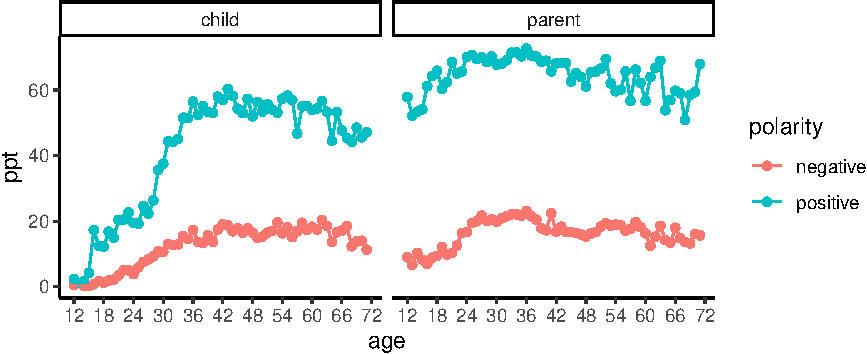
\includegraphics{negation_production_files/figure-latex/auxRelFreq-1.pdf}
\caption{\label{fig:auxRelFreq}Relative frequency of positive auxiliary forms such as \emph{do}, \emph{are}, and \emph{can} as well as their contracted negative form with \emph{nt} in the speech of parents and children.}
\end{figure}

\begin{verbatim}
## Warning: Ignoring unknown aesthetics: fill
\end{verbatim}

\begin{figure}
\centering
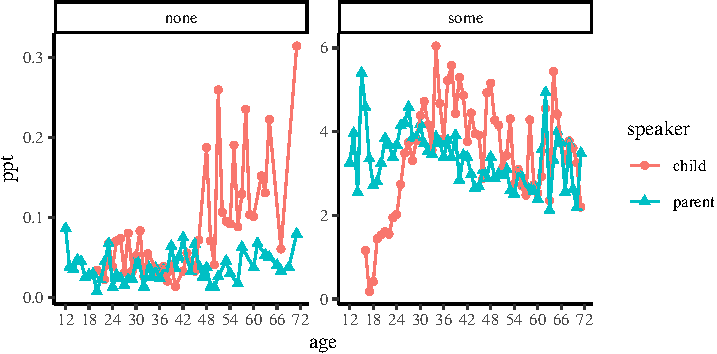
\includegraphics{negation_production_files/figure-latex/quantifiers-1.pdf}
\caption{\label{fig:quantifiers}Relative frequency of positive and negative quantifeirs.}
\end{figure}

\hypertarget{conclusions}{%
\subsection{Conclusions}\label{conclusions}}

Essentially the answers to these questions:

\begin{itemize}
\tightlist
\item
  What is the overall trajectory of negative forms in child production?

  \begin{itemize}
  \tightlist
  \item
    Does the development of negation follow a no \textgreater{} not \textgreater{} nt cline? (Cameron-faulkner et al)
  \item
    How many children are found to produce no/not/nt at each age?
  \end{itemize}
\item
  Do positive variants of the negative constructions exist too?

  \begin{itemize}
  \tightlist
  \item
    Are early \enquote{can't} and \enquote{don't} examples unanalyzed wholes? (Klima \& Bellugi 1966; Bloom 1970) Do children produce \enquote{can't} and \enquote{don't} before using \enquote{do} and \enquote{can}?
  \end{itemize}
\item
  Proportion of no vs.~not vs.~nt broken down by mean length of utterance

  \begin{itemize}
  \tightlist
  \item
    instead of age, put mean length of utterance on the x axis?
  \end{itemize}
\end{itemize}

\hypertarget{study-2-early-productions}{%
\section{Study 2: Early Productions}\label{study-2-early-productions}}

\hypertarget{participants}{%
\subsection{Participants}\label{participants}}

\hypertarget{material}{%
\subsection{Material}\label{material}}

\hypertarget{procedure-1}{%
\subsection{Procedure}\label{procedure-1}}

\hypertarget{data-analysis}{%
\subsection{Data analysis}\label{data-analysis}}

\hypertarget{results-1}{%
\section{Results}\label{results-1}}
>>>>>>> 9cd6424fe63fc80f114c1ca04fb952c90eaf9aee

\hypertarget{discussion}{%
\section{Discussion}\label{discussion}}

\newpage

\hypertarget{references}{%
\section{References}\label{references}}

\begingroup
\setlength{\parindent}{-0.5in}
\setlength{\leftskip}{0.5in}

\endgroup

\hypertarget{refs}{}
\leavevmode\hypertarget{ref-cameron2007part}{}%
Cameron-Faulkner, T., Lieven, E., \& Theakston, A. (2007). What part of no do children not understand? A usage-based account of multiword negation. \emph{Journal of Child Language}, \emph{34}(2), 251--282.

\leavevmode\hypertarget{ref-macwhinney2000childes}{}%
MacWhinney, B. (2000). \emph{The CHILDES project: The database} (Vol. 2). Mahwah, NJ: Erlbaum.

\leavevmode\hypertarget{ref-sanchez2018childes}{}%
Sanchez, A., Meylan, S., Braginsky, M., MacDonald, K., Yurovsky, D., \& Frank, M. C. (2018). Childes-db: A flexible and reproducible interface to the child language data exchange system. PsyArXiv. Retrieved from \url{psyarxiv.com/93mwx}


\end{document}
